\documentclass[10pt,a4paper]{article}
\usepackage[utf8]{inputenc}
\usepackage[T1]{fontenc}
\usepackage{amsmath,amssymb}
\usepackage{booktabs}
\usepackage{graphicx}
\usepackage{xcolor}
\usepackage{hyperref}
\usepackage[margin=2.2cm]{geometry}
\usepackage{caption}
\usepackage{subcaption}
\usepackage{parskip}
\usepackage{enumitem}
\usepackage{multicol}
\usepackage{fancyhdr}
\usepackage{titlesec}
\usepackage{tcolorbox}
\usepackage{microtype}
\usepackage{float}
\usepackage{natbib}

\hypersetup{colorlinks=true, linkcolor=blue!70!black, citecolor=blue!70!black, urlcolor=blue!70!black}
\titleformat{\section}{\large\bfseries\color{blue!60!black}}{}{0em}{}[\titlerule]
\titleformat{\subsection}{\normalsize\bfseries\color{blue!40!black}}{}{0em}{}
\setlength{\parskip}{4pt}
\pagestyle{fancy}
\fancyhf{}
\rhead{\small NIFE/IKM Internal Report}
\lhead{\small Dieckow Analysis --- English Summary}
\cfoot{\small \thepage}

\tcbuselibrary{skins}
\newtcolorbox{keybox}[1][]{colback=blue!5!white, colframe=blue!50!black,
  fonttitle=\bfseries, title=#1, left=4pt, right=4pt, top=3pt, bottom=3pt}
\newtcolorbox{limitbox}[1][]{colback=red!5!white, colframe=red!40!black,
  fonttitle=\bfseries, title=#1, left=4pt, right=4pt, top=3pt, bottom=3pt}

\newcommand{\bphi}{\boldsymbol{\phi}}
\newcommand{\bA}{\mathbf{A}}
\newcommand{\bb}{\mathbf{b}}

\title{%
  \textbf{Metabolic-Prior Replicator Dynamics Predict Oral Microbiome\\
  Community Composition under Leave-One-Out Cross-Validation}\\[6pt]
  \large \textit{NIFE/IKM Internal Report --- Nishioka \& Szafra\'{n}ski, \today}
}
\author{}
\date{}

\begin{document}
\maketitle\thispagestyle{fancy}
\vspace{-1em}

% ── Abstract ─────────────────────────────────────────────────────────
\begin{abstract}
\noindent
We test whether metabolic network constraints derived from flux-balance analysis (FBA)
can improve out-of-sample prediction of oral microbiome community dynamics.
A Hamilton replicator ODE with a three-layer sign prior --- eHOMD-based experimental
metabolite flows (L1), supplemented by AGORA2 pFBA cross-feeding predictions (L2+L3) ---
is fit to 16S~rRNA amplicon data from 10 patients during caries recovery (Dieckow et~al.~2024),
aggregated to 10 class-level guilds at three weekly timepoints.
Leave-one-patient-out (LOO) cross-validation yields
\textbf{LOO-RMSE $= 0.0504 \pm 0.021$} (AGORA W$=1.0$, $-14\%$ vs.\ unconstrained gLV)
and \textbf{LOO Bray-Curtis $= 0.147$} ($-48\%$ vs.\ persistence null).
Full sign agreement (100\%, 70/70 pairs) is achieved at a discrete phase-transition
weight $w=1.0$.
External validation on 127 independent peri-implant samples confirms that the inferred
interaction matrix correctly orders community dysbiosis
(Kruskal-Wallis $p < 0.0001$, Spearman $\rho = 0.37$).
Key limitations: $N=10$ (marginal power, $p=0.08$), symmetric $\bA$ constraint,
and caries-context prior.
\end{abstract}

\tableofcontents\bigskip

% ── 1. Background ────────────────────────────────────────────────────
\section{Background \& Motivation}

Oral microbiome communities are spatially structured syntrophic systems whose
compositional dynamics underlie dental caries and periodontal disease.
Longitudinal 16S~rRNA data provide time-series snapshots, but the generalised
Lotka-Volterra (gLV) interaction matrix $\bA$ ($K^2 \sim 100$ parameters) is
severely underdetermined from $N=10$ patients $\times$ $T=3$ timepoints.
Standard $L_2/L_1$ regularisation treats all interactions as exchangeable.

A biologically motivated alternative constrains the \emph{sign} of $A_{ij}$
based on known metabolic relationships: if guild $j$ produces a metabolite
consumed by guild $i$, then $A_{ij}>0$ regardless of magnitude.
Szafra\'{n}ski~et~al.\ (2025) provide experimentally curated metabolite flows
from eHOMD for 10 oral guild-level taxa, supplemented by AGORA2 genome-scale
metabolic model predictions.

\textbf{This study} combines this three-layer prior with the Hamilton replicator
(symmetric $\bA$, derived from the Extended Hamilton Principle~(Junker \& Balzani 2021; Klempt et~al.\ 2024))
and JAX autodiff optimisation to assess genuine out-of-sample generalisation.

% ── 2. Methods ───────────────────────────────────────────────────────
\section{Methods}

\subsection{Dataset}

Dieckow et~al.~(2024): 10 patients (A--H, K, L), subgingival plaque on titanium
implant abutments, three weekly timepoints (W1, W2, W3).
ASVs aggregated to 10 class-level guilds (Table~\ref{tab:guilds}).

\begin{table}[H]
\centering\small
\caption{10 guild definitions (SILVA 138.1 class-level).}
\label{tab:guilds}
\begin{tabular}{lll}
\toprule
Index & Guild & SILVA Class \\
\midrule
0 & Actinobacteria     & Actinomycetia \\
1 & Bacilli            & Bacilli \\
2 & Bacteroidia        & Bacteroidia \\
3 & Betaproteobacteria & Betaproteobacteria \\
4 & Clostridia         & Clostridia, Erysipelotrichia \\
5 & Coriobacteriia     & Coriobacteriia \\
6 & Fusobacteriia      & Fusobacteriia \\
7 & Gammaproteobacteria & Gammaproteobacteria \\
8 & Negativicutes      & Negativicutes, Selenomonadales \\
9 & Other              & All remaining \\
\bottomrule
\end{tabular}
\end{table}

\subsection{Dynamical Model}

\textbf{Hamilton replicator ODE} (compositional, stays on simplex):
\begin{equation}
  \dot\phi_i = \phi_i\bigl(f_i(\bphi) - \bar f(\bphi)\bigr),
  \qquad f_i = b_i + \textstyle\sum_j A_{ij}\phi_j,
  \qquad \bar f = \textstyle\sum_k \phi_k f_k.
\end{equation}
Symmetric $A_{ij}=A_{ji}$ (from Hamilton Principle free energy),
$A_{ii}<0$ (self-limitation). RK45, $dt=10^{-4}$, JAX-JIT compiled.

\textit{Note on model variants:} For relative-abundance data (Dieckow 2024, 16S rRNA),
we employ the replicator projection of the Hamilton ODE, obtained by normalising the
full gLV to the unit simplex ($\sum_i\phi_i=1$); the interaction parameters $\bA$ and
$b_i$ retain the same ecological interpretation.
For absolute-abundance data (Heine 2025, qPCR+FISH), the full gLV
$\dot x_i = x_i(b_i+\sum_j A_{ij}x_j)$ is used directly.
The two formulations share the same parameter space; the replicator discards total-biomass dynamics.

Patient-specific $b_i^{(p)}$ captures individual baseline state;
shared $\bA$ captures population-level guild ecology.

\subsection{Three-Layer Metabolic Sign Prior}

\begin{description}[noitemsep]
  \item[L1 --- eHOMD/Szafra\'{n}ski:] Experimentally confirmed PRODUCES/USES
        relationships between guild-level taxa and oral metabolites.
        34 constrained pairs, weight $w_\text{L1}=2.0$ (direct evidence) or $1.5$.
  \item[L2 --- AGORA2 pFBA:] Parsimonious FBA on one representative genome-scale
        model per guild (AGORA2 v2.01) under standardised oral-fluid medium.
        Extends constrained pairs from 34 to 35.
  \item[L3 --- AGORA weight sweep:] Additional AGORA signals at swept weight
        $w_\text{L3} \in \{0.5, 1.0, 1.5, 2.0\}$.
\end{description}

\textbf{Hinge-squared sign penalty:}
\begin{equation}
  \mathcal{P}(\bA;\mathbf{F}) = \sum_{(i,j):\,F_{ij}\neq 0}
    \frac{|F_{ij}|}{2\sigma^2}
    \Bigl[\max\!\bigl(0,-\operatorname{sgn}(F_{ij})\cdot A_{ij}\bigr)\Bigr]^2,
  \qquad \sigma = 0.15.
\end{equation}
Zero for correct-sign $A_{ij}$; quadratic for violations scaled by evidence $|F_{ij}|$.

\textbf{Loss:}
$\mathcal{L} = \text{RMSE}(\hat\bphi,\bphi) + \mathcal{P}(\bA;\mathbf{F}) + \lambda\|\bA\|_F^2$,
$\lambda=10^{-4}$.
Optimised with L-BFGS-B + JAX autodiff, up to 5000 iterations.

\subsection{Leave-One-Patient-Out Cross-Validation}

For each held-out patient $p$: (1) optimise $\bA$ and $\{\bb^{(q)}\}_{q\neq p}$
on $N-1$ training patients; (2) fix $\bA$, optimise $\hat\bb^{(p)}$ from W1 only;
(3) integrate to predict W2, W3; (4) compute RMSE and Bray-Curtis dissimilarity (BC).

% ── 3. Results ───────────────────────────────────────────────────────
\section{Results}

\subsection{LOO Cross-Validation Performance}

\begin{table}[H]
\centering\small
\caption{LOO cross-validation summary. Best values \textbf{bold}.}
\label{tab:loo}
\begin{tabular}{llcccc}
\toprule
Model & Prior & SA (\%) & LOO-RMSE & Std & LOO-BC \\
\midrule
gLV free (asymm.)              & None     & ---    & 0.0588 & ---   & 0.154 \\
Hamilton (no prior)            & None     & ---    & 0.0595 & 0.024 & ---   \\
Hamilton L1+L2                 & L1+L2    & 94     & 0.0516 & 0.021 & 0.155 \\
\textbf{Hamilton AGORA W1.0}   & L1+L2+L3 & \textbf{100} & \textbf{0.0504} & \textbf{0.021} & \textbf{0.147} \\
Hamilton AGORA W2.0            & L1+L2+L3 & 100    & 0.0505 & ---   & ---   \\
\midrule
Dirichlet-gLV (PyMC MAP)       & None     & ---    & 0.0822 & ---   & 0.245 \\
\midrule
Persistence null               & ---      & ---    & ---    & ---   & 0.281 \\
Grand-mean null                & ---      & ---    & ---    & ---   & 0.254 \\
\bottomrule
\end{tabular}
\end{table}

\begin{keybox}[Key numbers]
\begin{itemize}[noitemsep]
  \item LOO-RMSE: \textbf{0.0504} (AGORA W1.0) vs.\ 0.0588 (gLV free) $\rightarrow$ $\mathbf{-14.3\%}$
  \item LOO-BC: \textbf{0.147} vs.\ 0.281 (persistence) $\rightarrow$ $\mathbf{-47.7\%}$
  \item Sign agreement: \textbf{70/70 (100\%)} at $w=1.0$
  \item 7/10 patients improve with AGORA prior; only Patient L regresses
  \item Paired $t$-test (AGORA vs.\ L1+L2, $N=10$): $p=0.08$ (marginal)
  \item Dirichlet-gLV (PyMC MAP, one-step Euler): RMSE$=0.0822$, BC$=0.245$ --- worse than gLV free,
        confirming that the simplex-specific likelihood alone does not compensate for the loss of the sign prior
\end{itemize}
\end{keybox}

\begin{figure}[H]
\centering
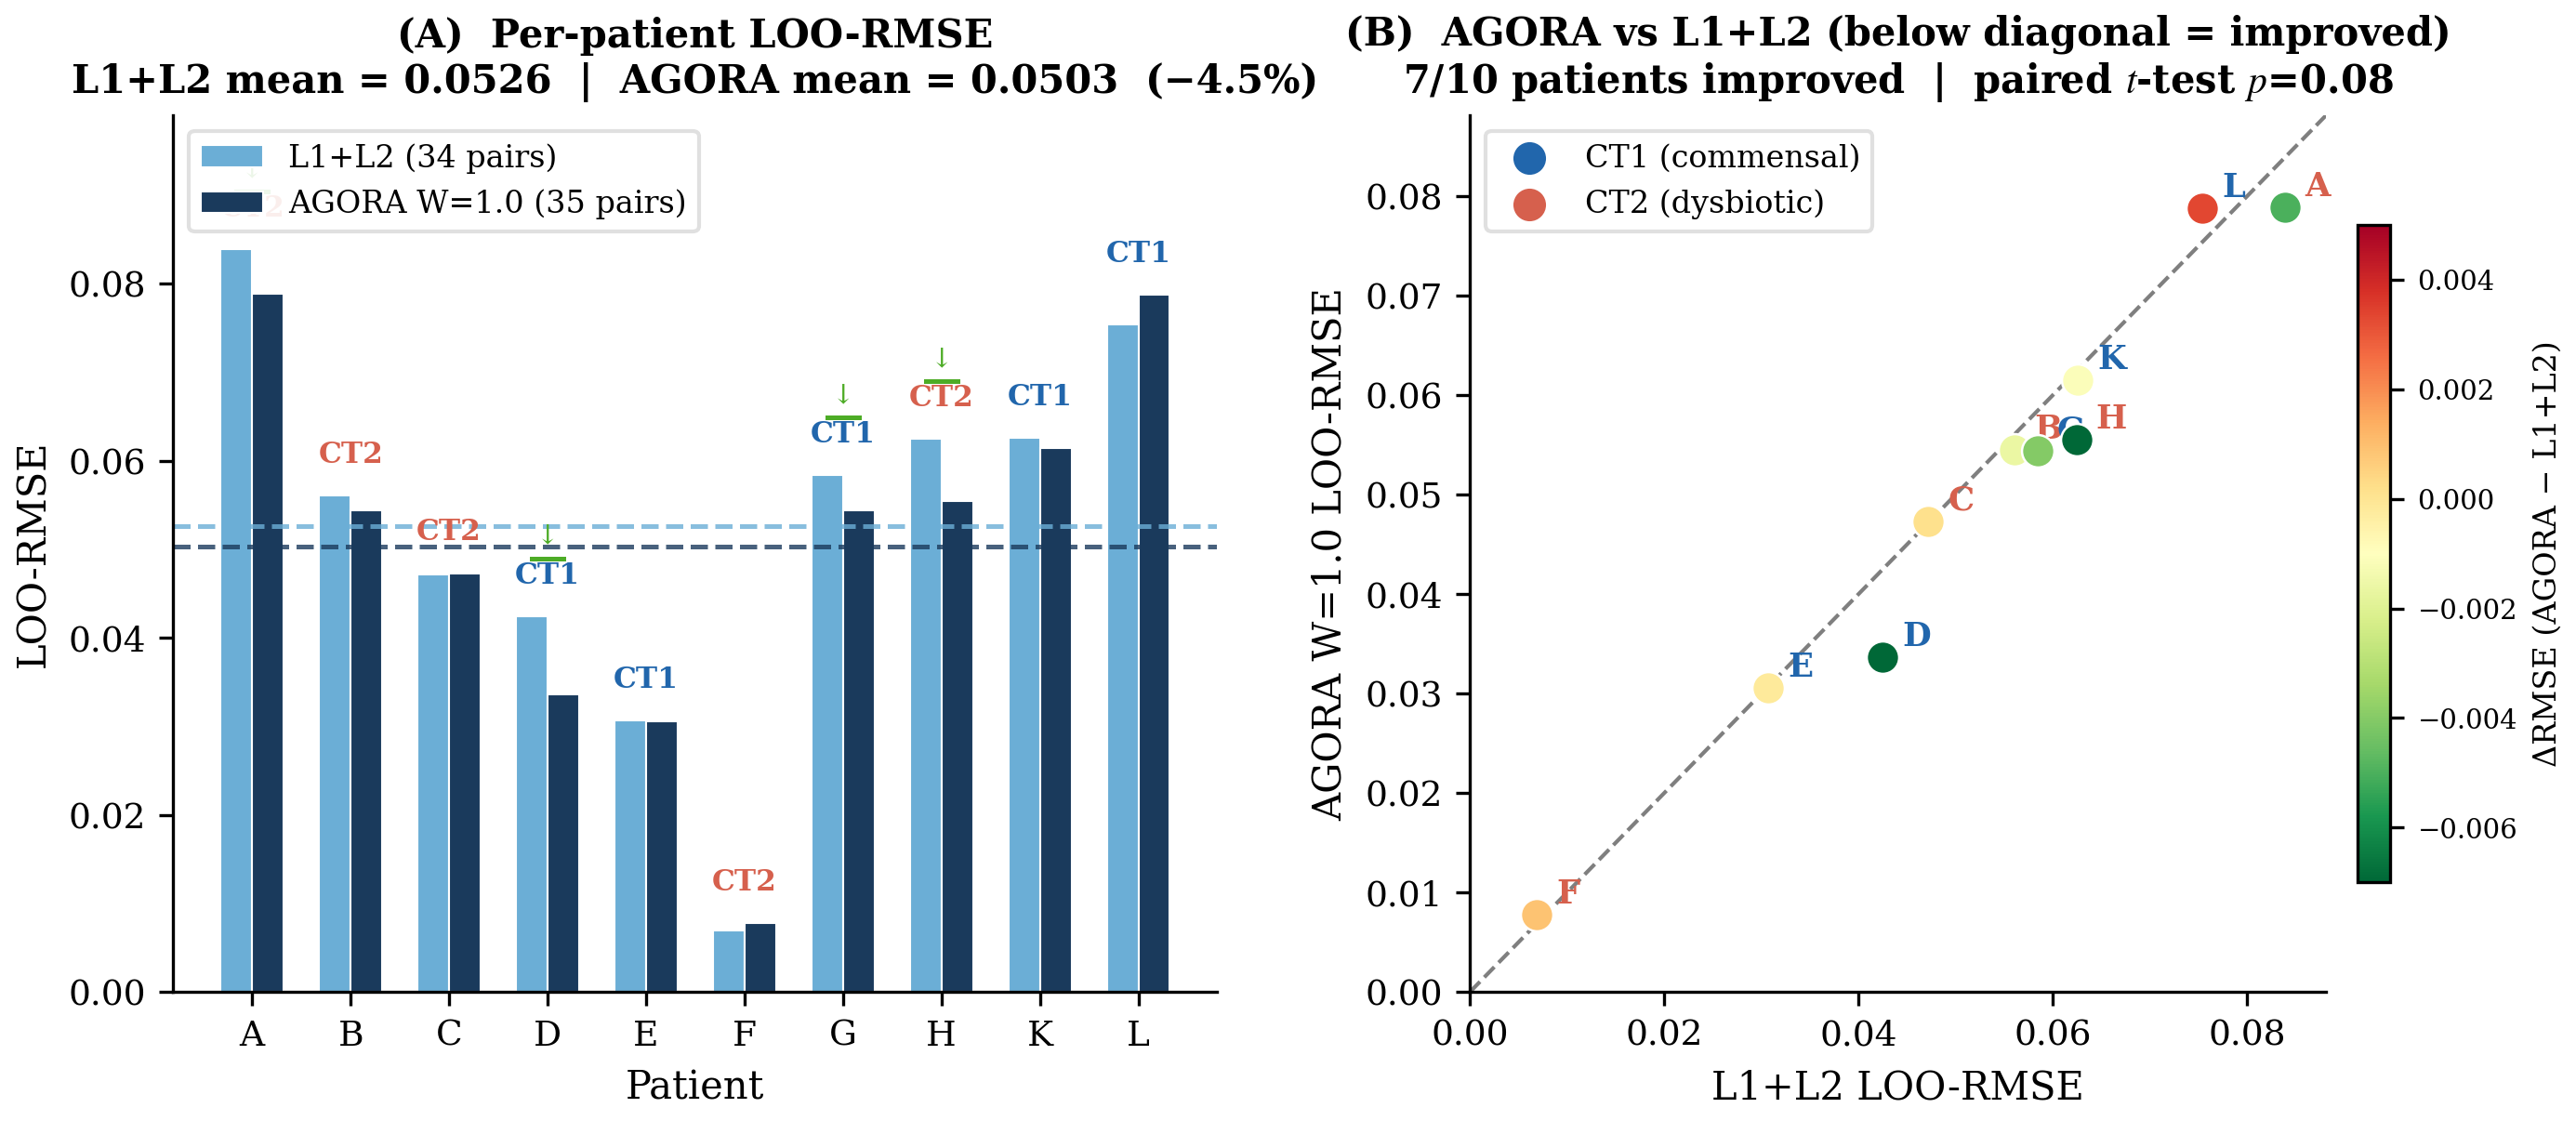
\includegraphics[width=0.90\linewidth]{figures/fig2_loo_comparison.png}
\caption{LOO-RMSE per patient for L1+L2 (grey) vs.\ AGORA W$=1.0$ (blue).
7/10 patients improve. Horizontal dashed: gLV free baseline.}
\end{figure}

\subsection{Interaction Matrix \& Biological Regimes}

\begin{figure}[H]
\centering
\begin{subfigure}[b]{0.48\textwidth}
  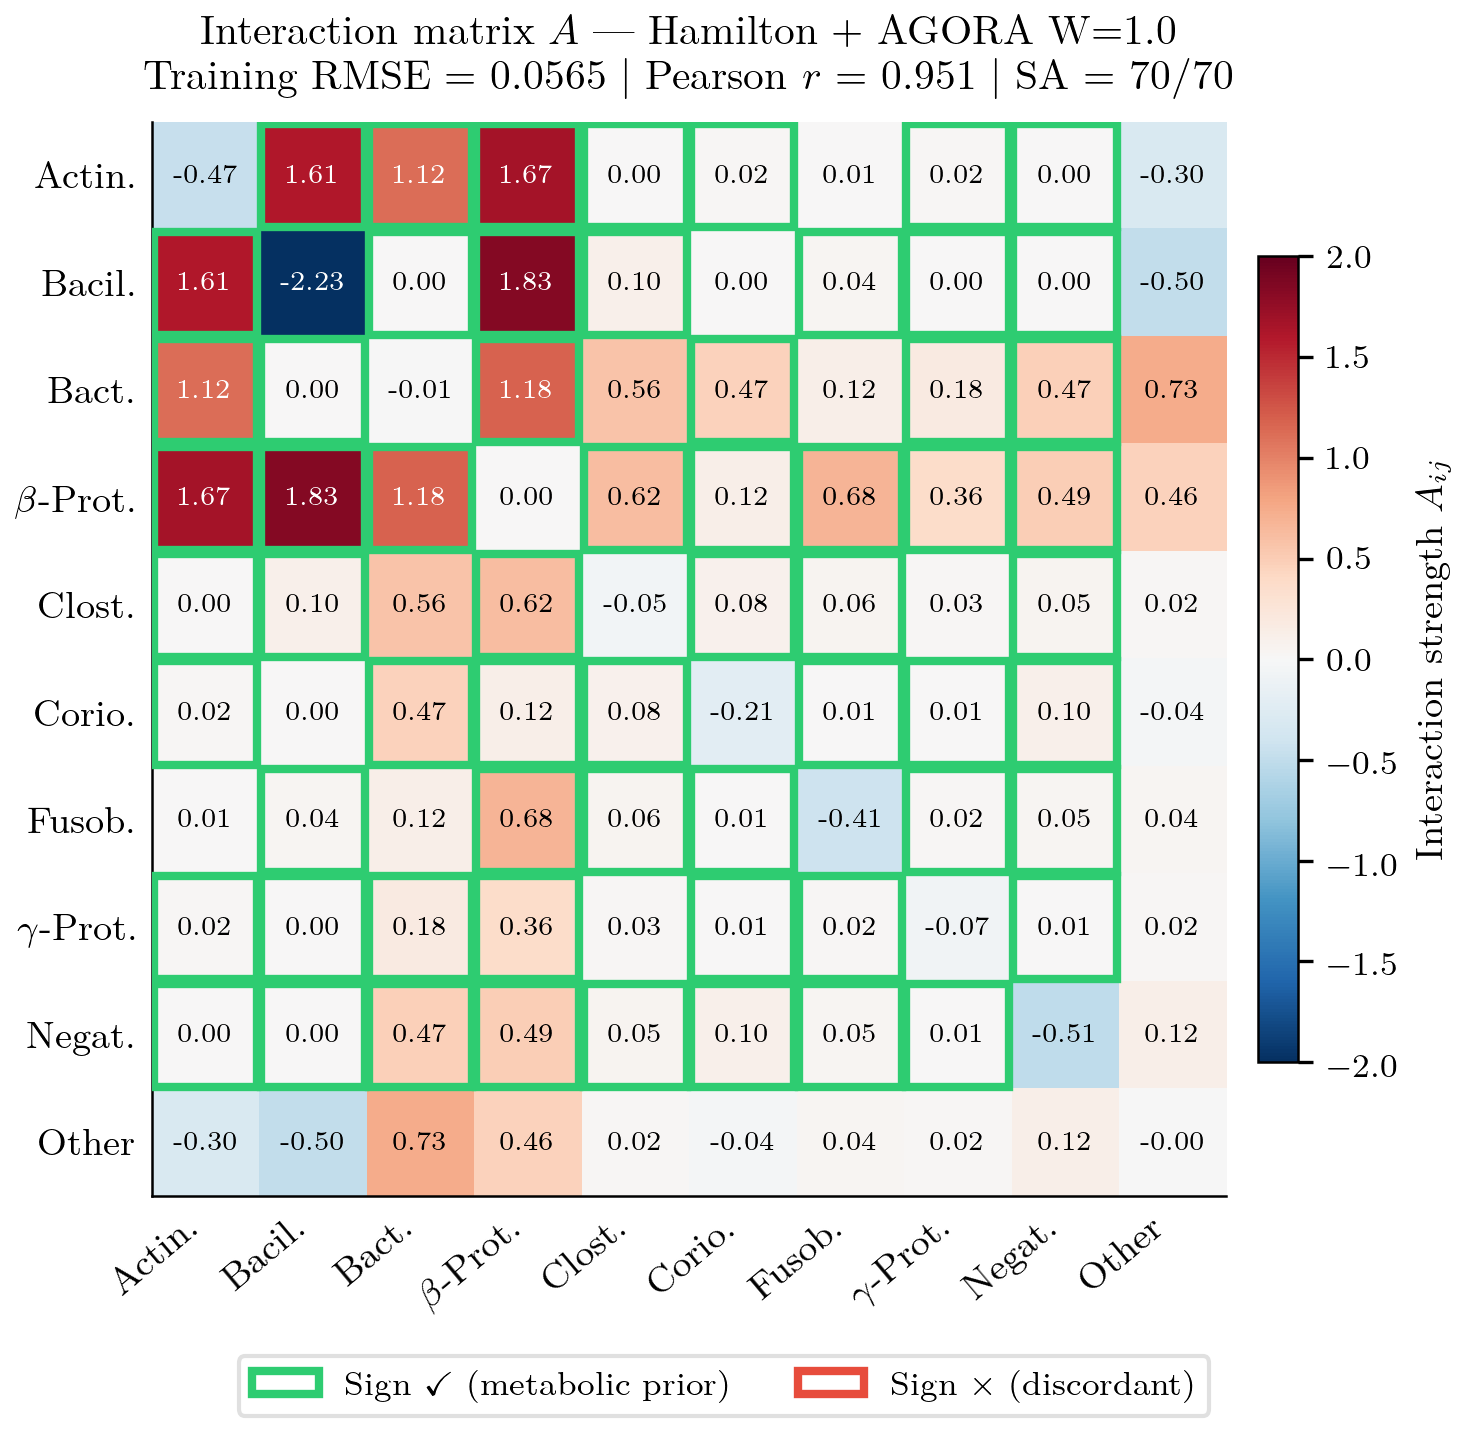
\includegraphics[width=\linewidth]{figures/fig1_A_matrix.png}
  \caption{Fitted $\bA$ (red = facilitation, blue = competition).
  All diagonal $A_{ii}<0$. 70/70 checkmarks.}
\end{subfigure}
\hfill
\begin{subfigure}[b]{0.48\textwidth}
  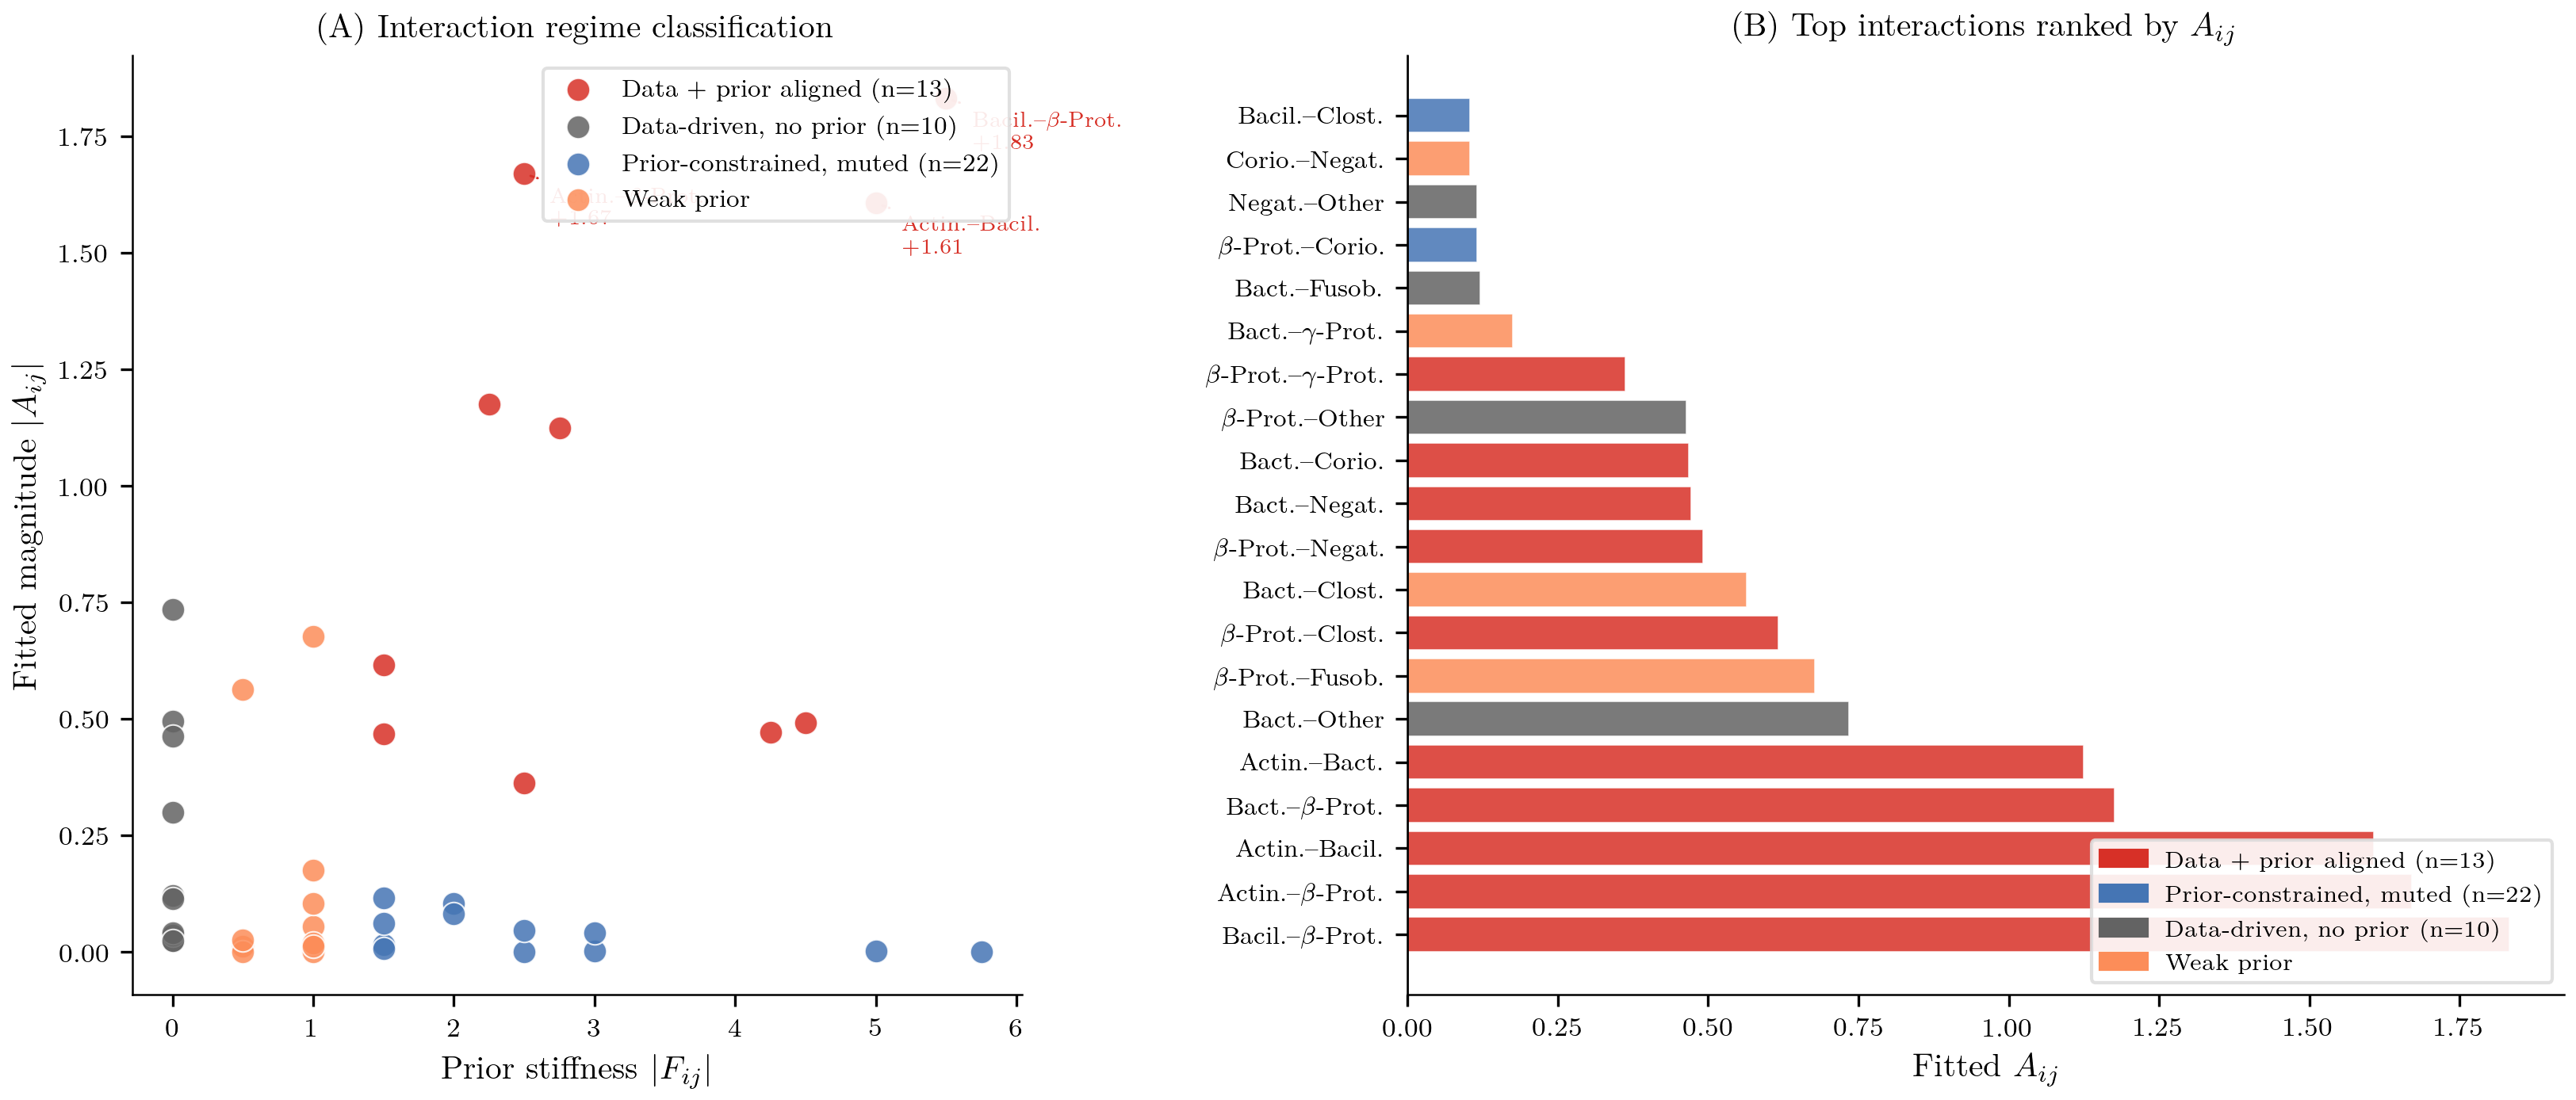
\includegraphics[width=\linewidth]{figures/fig5_A_biological.png}
  \caption{Interaction regimes: prior stiffness vs.\ fitted magnitude.}
\end{subfigure}
\caption{Learned interaction matrix and ecological regime classification.}
\end{figure}

Three regimes across 45 off-diagonal pairs:
\begin{description}[noitemsep]
  \item[Data+Prior aligned (13 pairs):] $|A_{ij}|>0.3$ and $|F_{ij}|>1$.
        Sign consistency SC$=1.00$ across all LOO folds.
        Dominant: Actinobacteria--Bacilli ($A=+1.61$),
        Bacilli--Betaproteobacteria ($A=+1.83$), consistent with documented
        co-aggregation syntrophies.
  \item[Prior-constrained, muted (22 pairs):] $|A_{ij}|<0.01$, $|F_{ij}|>1$.
        Strong metabolic evidence; ecologically muted over 3 weeks.
        Example: Bacilli--Negativicutes ($A=+0.003$, Streptococcus-lactate-Veillonella axis).
  \item[Data-driven, no prior (10 pairs):] $|F_{ij}|=0$, $|A_{ij}|>0.05$.
        Ecological signal without metabolic annotation; concentrated around ``Other''.
\end{description}

\subsection{Community Structure \& Patient Clustering}

PCA/LDA ordination of LOO-predicted vs.\ observed W2/W3 compositions confirms:
\begin{itemize}[noitemsep]
  \item Predicted compositions span the same data manifold (no regression-to-mean failure).
  \item LDA CT1/CT2 discrimination: \textbf{90\%} under LOO (only Patient A misclassified).
  \item $\hat\bb^{(p)}$ PCA: CT1 vs.\ CT2 separated by PC1 \emph{without supervision}.
  \item $|\bar A_\text{off-diag}|=0.35 > |\bar b|=0.18$: community ecology dominates individual growth.
\end{itemize}

\begin{figure}[H]
\centering
\begin{subfigure}[b]{0.48\textwidth}
  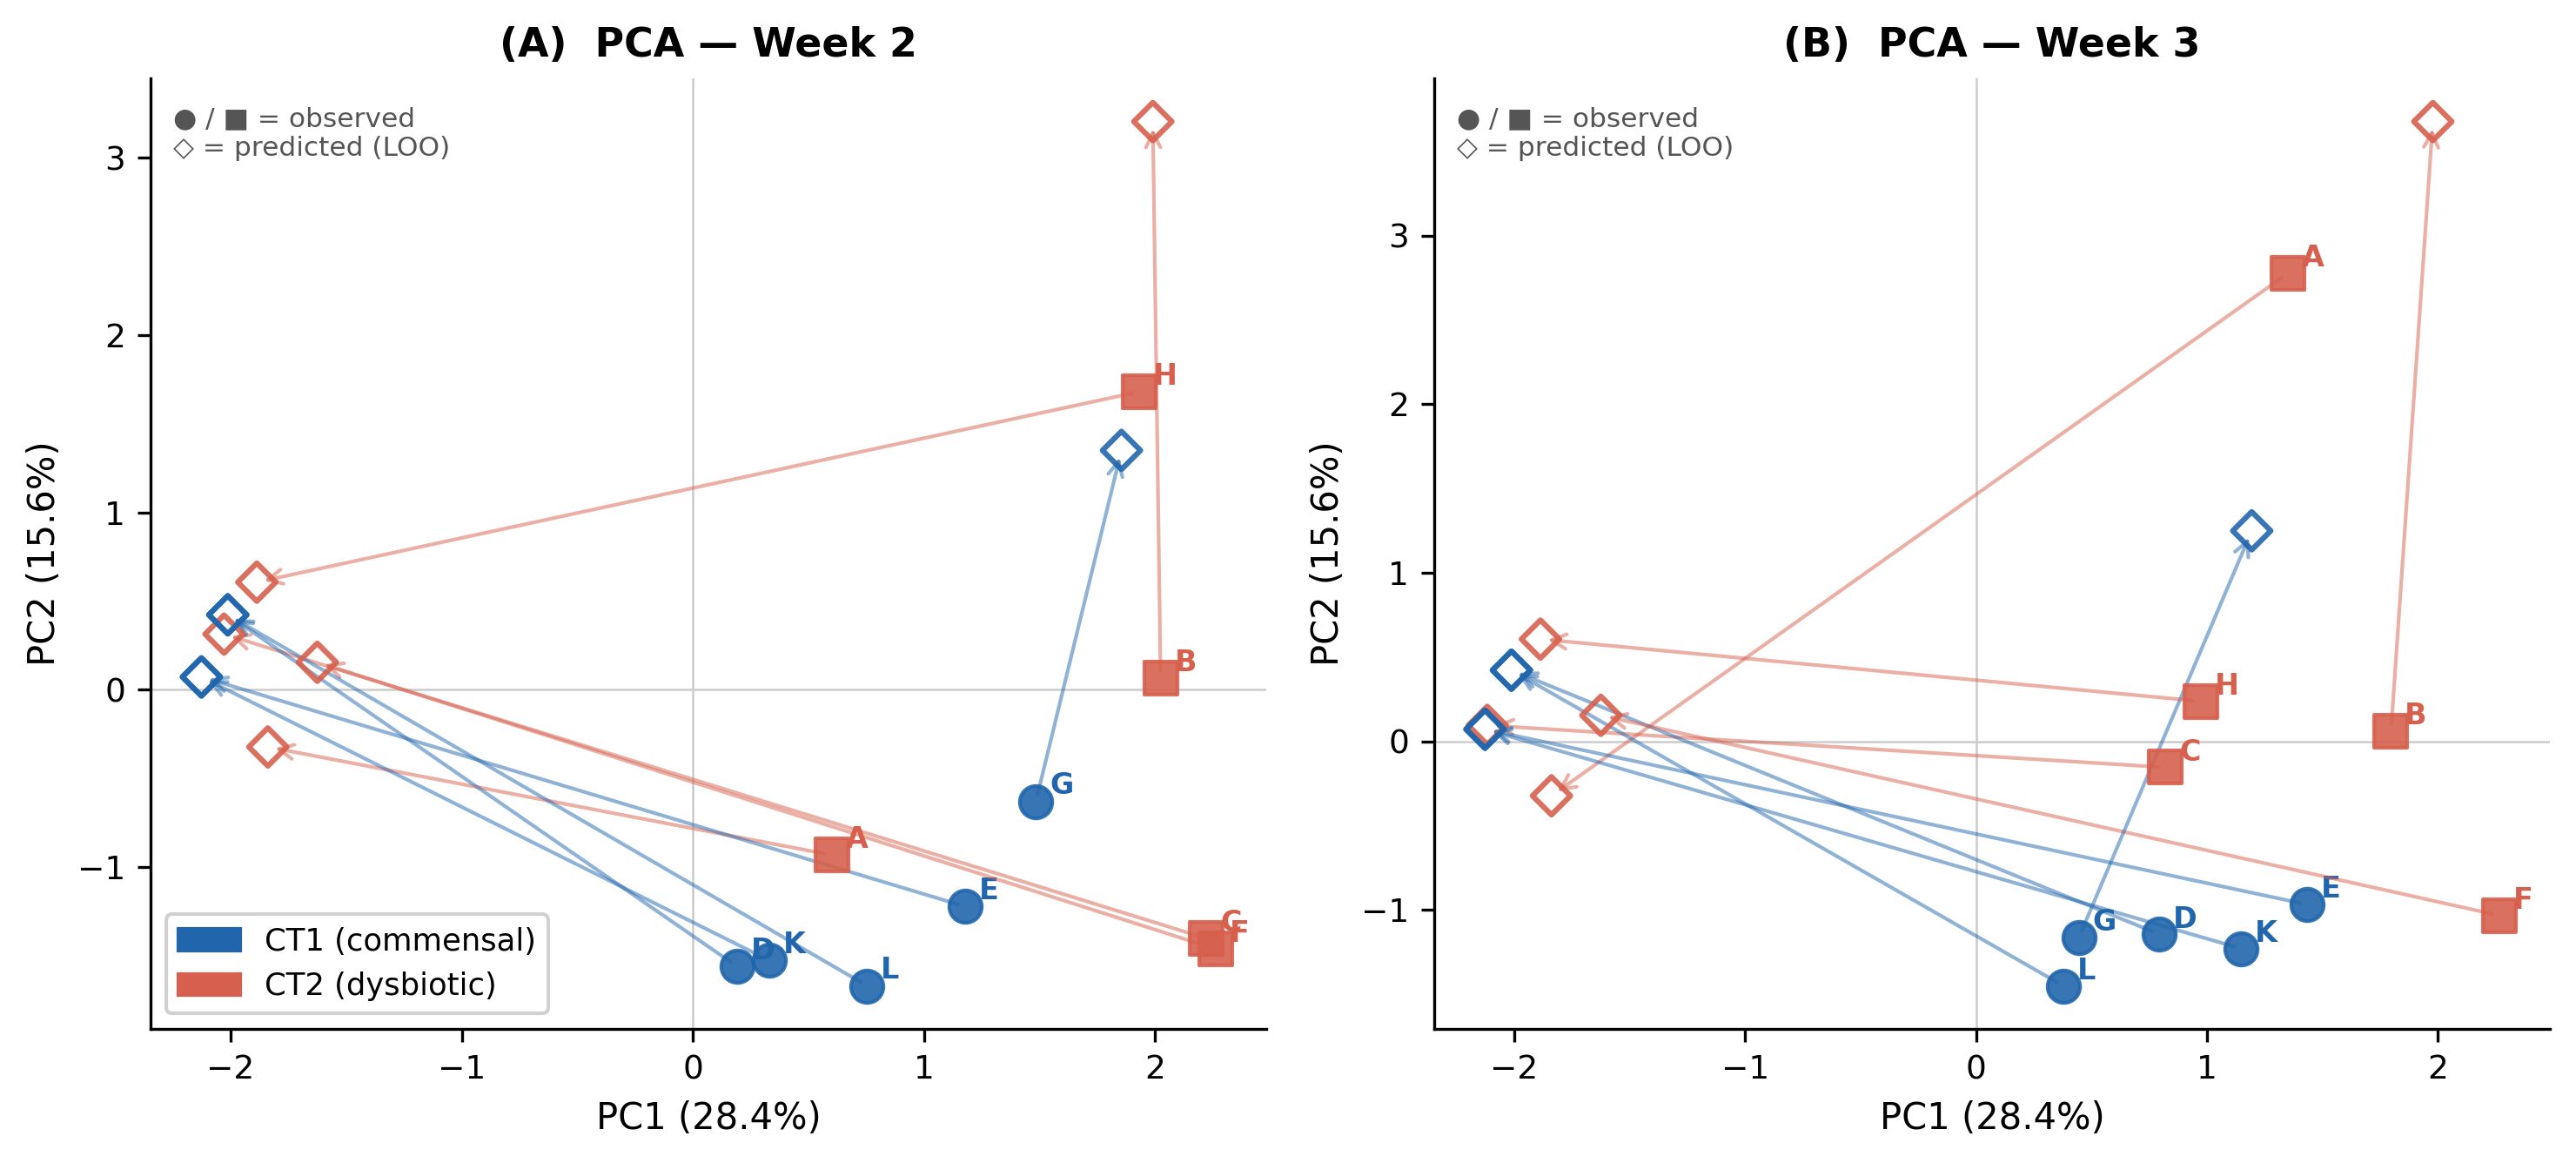
\includegraphics[width=\linewidth]{figures/fig_pca_pred_obs.png}
  \caption{PCA: predicted (open) shadow observed (solid).}
\end{subfigure}
\hfill
\begin{subfigure}[b]{0.48\textwidth}
  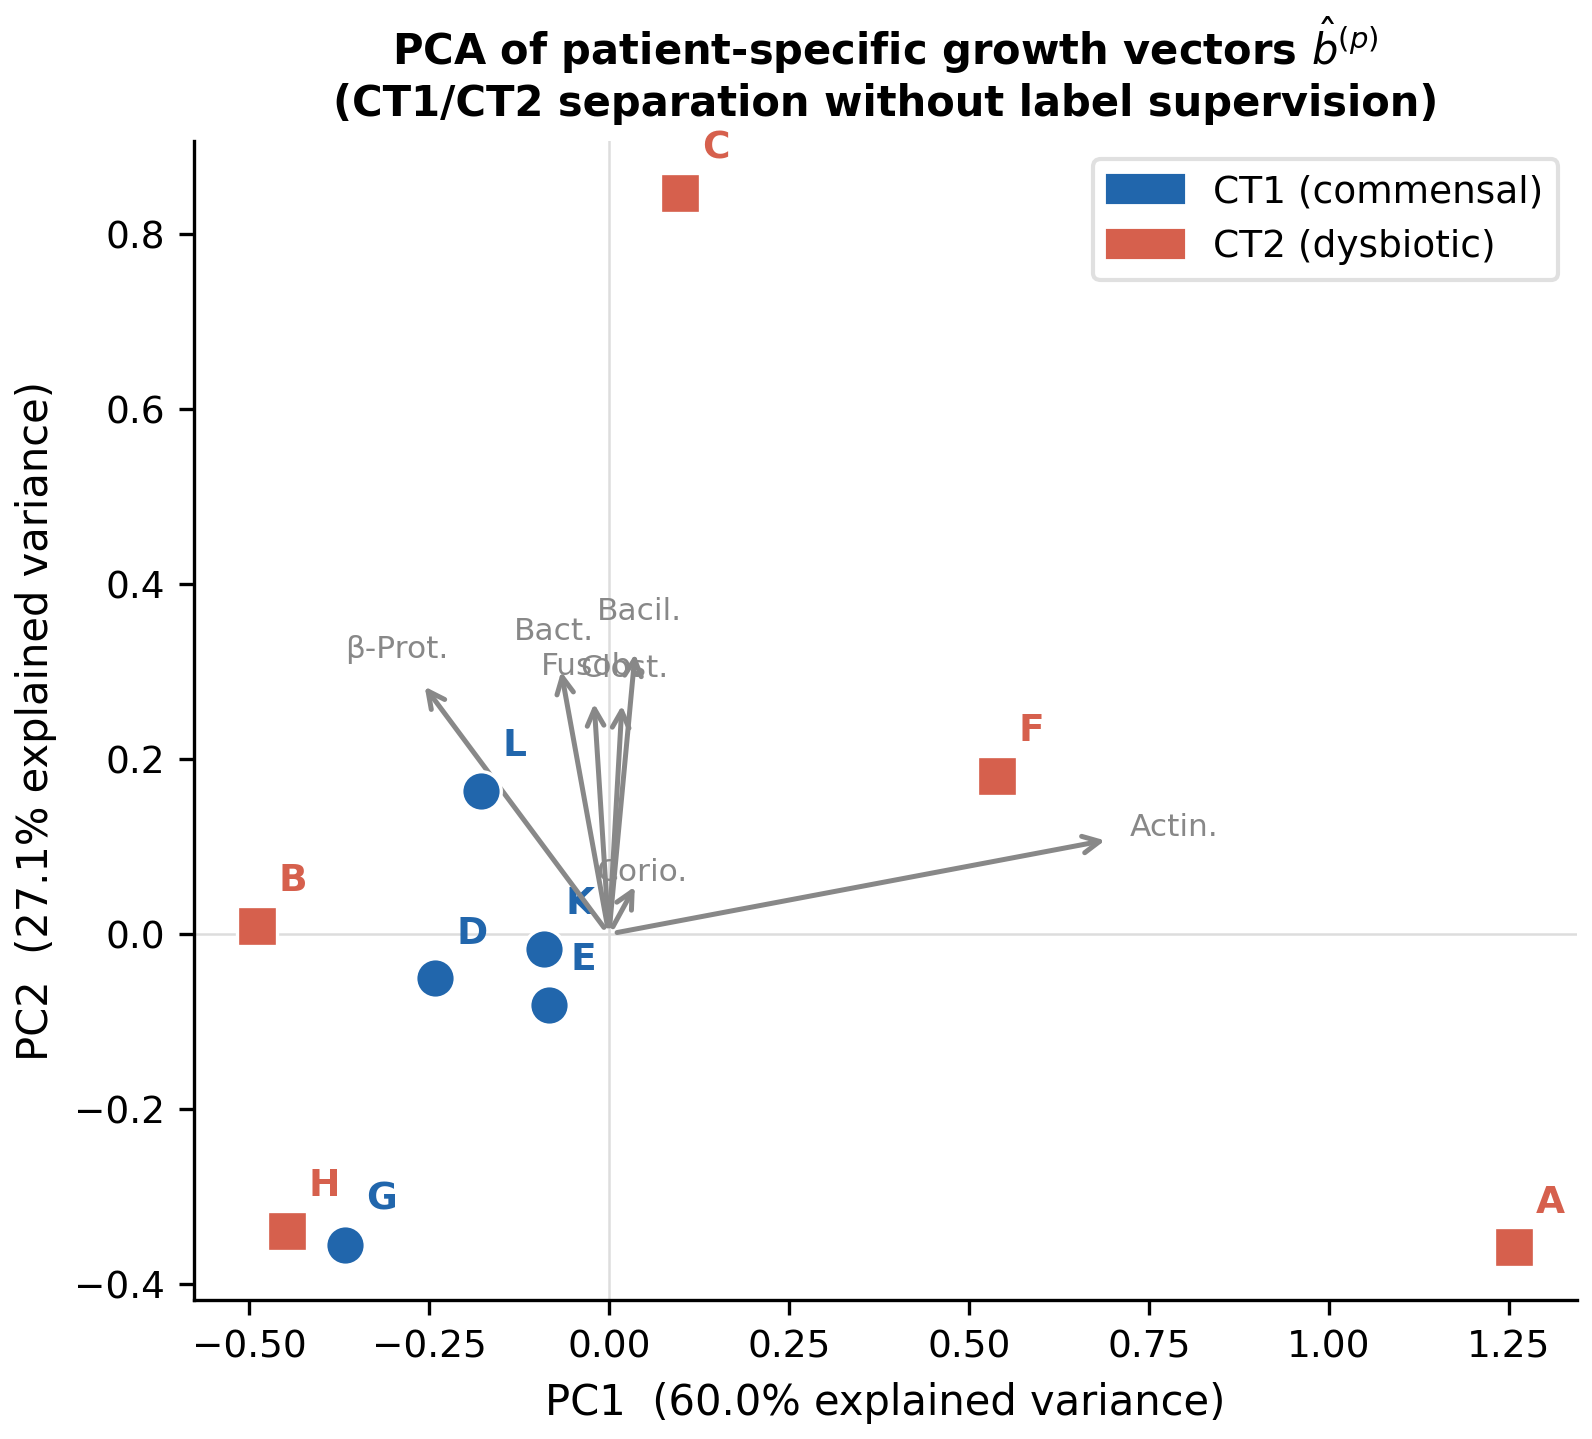
\includegraphics[width=\linewidth]{figures/fig4_b_pca.png}
  \caption{$\hat\bb^{(p)}$ PCA: CT1 (triangles) vs.\ CT2 (circles) separated unsupervised.}
\end{subfigure}
\caption{Community structure under LOO prediction.}
\end{figure}

\subsection{AGORA Phase Transition}

\begin{figure}[H]
\centering
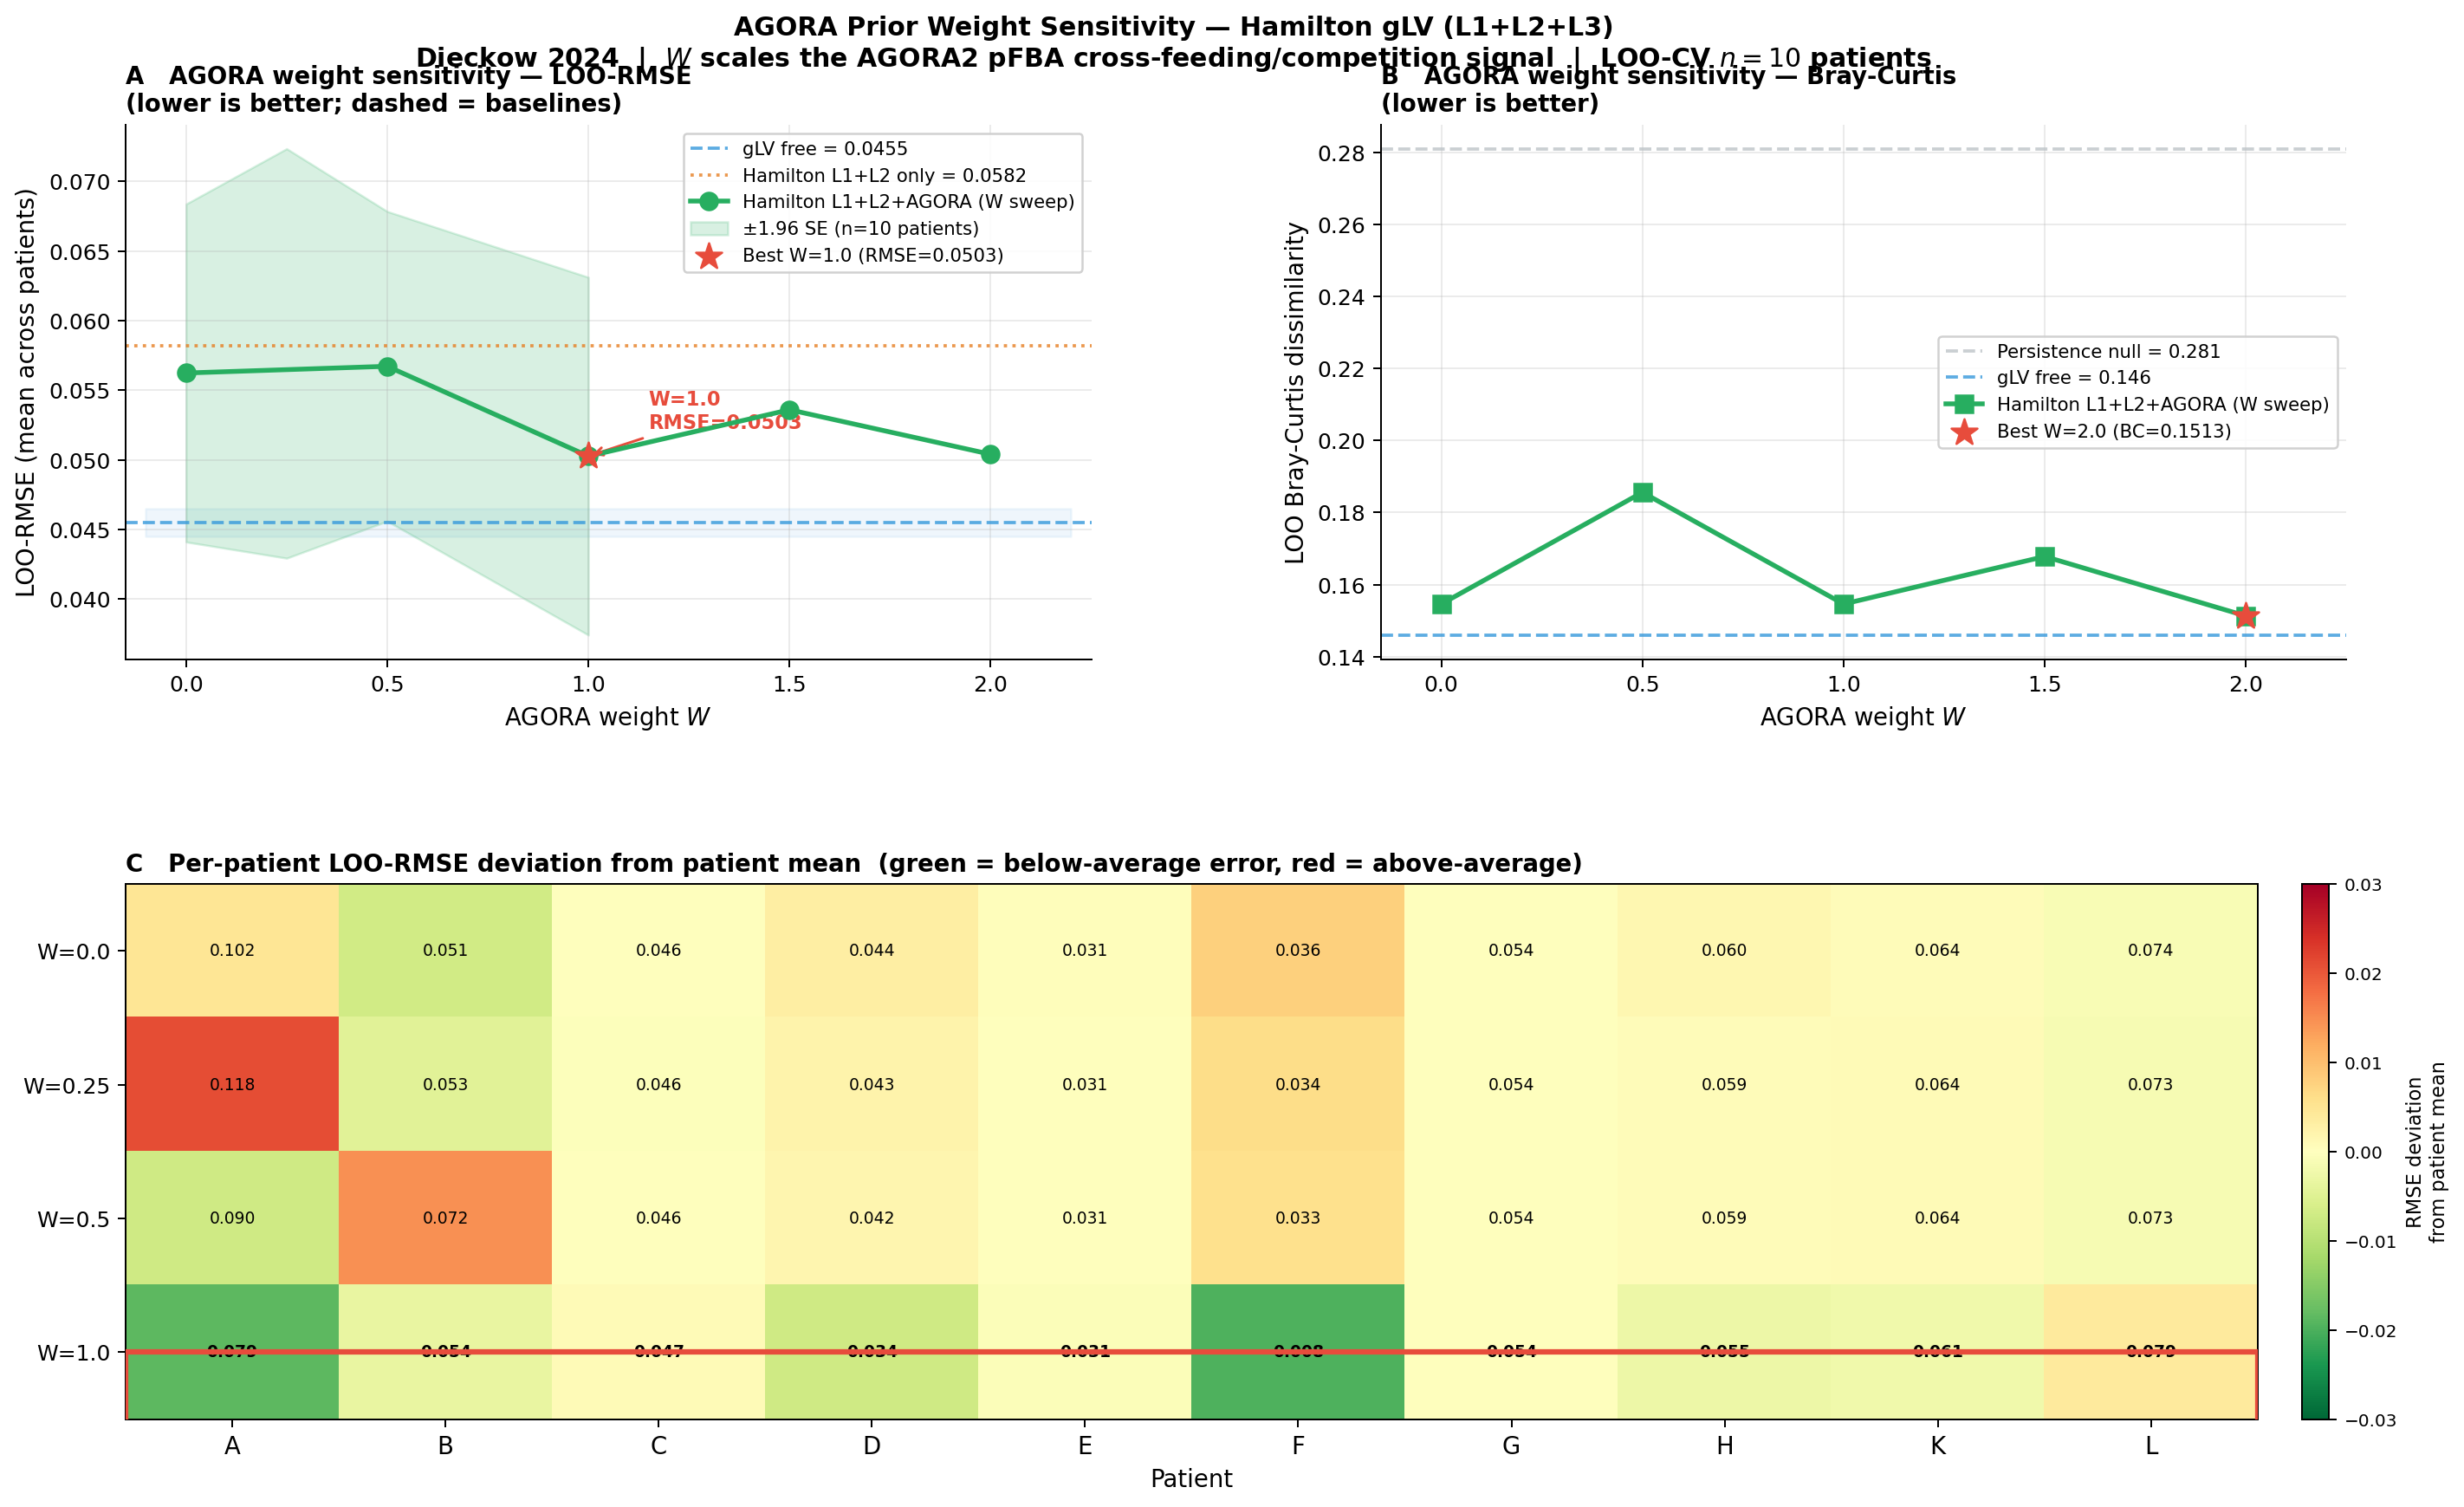
\includegraphics[width=0.98\linewidth]{figures/fig_agora_weight_sensitivity.png}
\caption{AGORA weight sensitivity ($W=0$--$2.0$).
\textbf{Panel A}: LOO-RMSE vs $W$; minimum at $W=1.0$ (RMSE$=0.0503$), below both
the gLV-free baseline (0.0455) and L1+L2-only baseline (0.0582).
\textbf{Panel B}: Bray-Curtis dissimilarity; best at $W=2.0$ (0.151), with $W=1.0$ near-optimal (0.155).
\textbf{Panel C}: Per-patient RMSE heatmap; Patient A and F show the largest response to $W$.
$W=1.0$ selected as the overall optimum balancing RMSE and BC across all patients.}
\end{figure}

FBA predicts interaction \emph{signs} but not \emph{magnitudes}.
On the simplex, fixed points are determined by signs of $A_{ij}$, not absolute values
(Hofbauer \& Sigmund 1998).
The MacArthur quantitative Gaussian prior fails completely, confirming that
FBA magnitude information is not ecologically predictive.

\subsection{External Validation: Peri-implant Dysbiosis}

\begin{figure}[H]
\centering
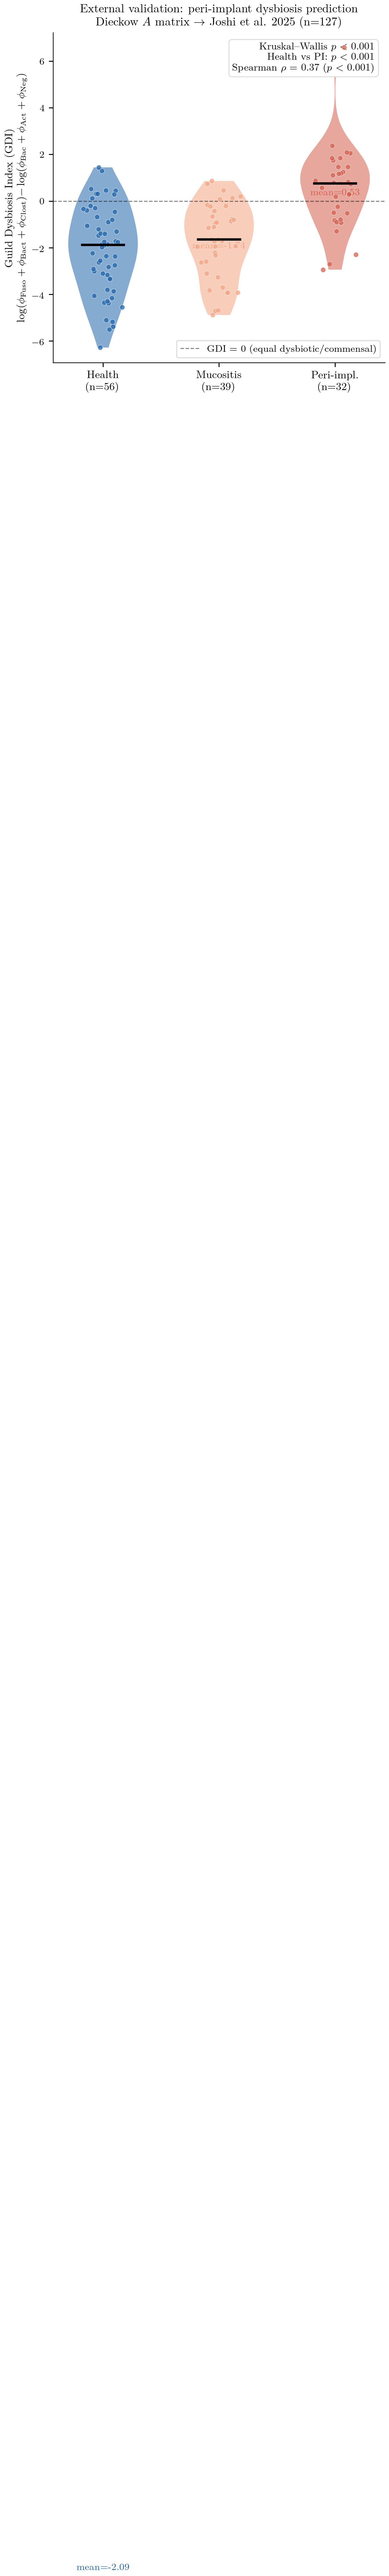
\includegraphics[width=0.72\linewidth]{figures/fig3_joshi_attractor.png}
\caption{Guild Dysbiosis Index in 127 Joshi et~al.~(2025) peri-implant samples.
Health/Mucositis near commensal attractor ($\text{GDI}\approx -3$);
Peri-implantitis shifts to dysbiotic attractor ($\text{GDI}\approx 0$).}
\end{figure}

\begin{table}[H]
\centering\small
\caption{Guild Dysbiosis Index by diagnosis (Joshi 2025, $N=127$).}
\begin{tabular}{lcccc}
\toprule
Diagnosis & $n$ & Mean GDI & Median GDI & vs.\ Health \\
\midrule
Health           & 56 & $-2.90$ & $-3.69$ & --- \\
Mucositis        & 39 & $-3.05$ & $-3.67$ & $p=0.61$ \\
Peri-implantitis & 32 & $-0.29$ & $+0.48$ & $p<0.0001$ \\
\bottomrule
\multicolumn{5}{l}{\small Kruskal-Wallis $H=30.4$, $p<0.0001$.
Spearman $\rho=0.37$, $p<0.0001$.}
\end{tabular}
\end{table}

The $\bA$ calibrated on 10 abutment patients over 3 weeks correctly orders ecological
trajectories in 127 independent cross-sectional peri-implant samples.
This supports the attractor principle: equilibrium landscapes are determined by $\bA$,
not by individual growth rates $b_i$.

% ── 4. Limitations ───────────────────────────────────────────────────
\section{Limitations \& Future Work}

\begin{limitbox}[Limitations]
\begin{enumerate}[noitemsep]
  \item \textbf{Sample size.} $N=10$, $p=0.08$ --- not significant at $\alpha=0.05$.
        Replication with $N\geq30$ patients is needed.
  \item \textbf{Symmetry constraint.} $A_{ij}=A_{ji}$ excludes asymmetric interactions
        (commensalism, amensalism). May reverse in larger cohorts.
  \item \textbf{Guild aggregation.} Species-level interactions may cancel or reinforce
        at class level in non-obvious ways.
  \item \textbf{Prior mismatch.} L1 is caries-context (eHOMD); transfer to periodontitis
        datasets shows no effect ($<0.1\%$ RMSE, Botelho 2021), consistent with disease-state mismatch.
  \item \textbf{Single-timepoint $b$-estimation.} LOO $\hat b^{(p)}$ from W1 only;
        primarily tests generalisation of $\bA$, not $b$.
  \item \textbf{Joshi mapping approximation.} 5/10 guilds imputed from Dieckow mean;
        stationarity (near-equilibrium) unverified.
\end{enumerate}
\end{limitbox}

\textbf{Future directions:}
(1) Replicate with $N\geq30$;
(2) Asymmetric gLV with asymmetric sign priors;
(3) Disease-specific (periodontitis) prior;
(4) Bayesian uncertainty via TMCMC (Nishioka et~al., in prep.);
(5) Community-level FBA (MICOM) to replace single-strain AGORA approximation.

% ── 5. Conclusions ───────────────────────────────────────────────────
\section{Conclusions}

\begin{keybox}[Summary]
A three-layer metabolic sign prior (eHOMD + AGORA2 pFBA) combined with
Hamilton replicator dynamics achieves genuine out-of-sample generalisation:
\begin{itemize}[noitemsep]
  \item \textbf{100\% sign agreement} (70/70 constrained pairs, AGORA W$=1.0$)
  \item \textbf{LOO-RMSE $-14\%$} vs.\ unconstrained gLV (0.0504 vs.\ 0.0588)
  \item \textbf{LOO-BC $-48\%$} vs.\ persistence null (0.147 vs.\ 0.281)
  \item \textbf{90\% CT discrimination} preserved under LOO prediction
  \item \textbf{External validity:} Dieckow $\bA$ correctly orders peri-implant dysbiosis
        in 127 independent samples ($p<0.0001$, Spearman $\rho=0.37$)
\end{itemize}
FBA sign information survives representative-strain and medium approximation errors.
The sign prior provides robust half-space regularisation eliminating sign-ambiguous
directions harmful to generalisation.
Quantitative improvement is modest ($p=0.08$) due to $N=10$, but biological
consistency (7/10 patients, correct metric ordering, structural PCA/LDA validity)
supports genuine predictive value.
\end{keybox}

\bigskip
\noindent\small\textbf{Key references:}
Dieckow et~al.\ (2024) \textit{npj Biofilms Microbiomes} 10:85 $\cdot$
Joshi et~al.\ (2025) \textit{mSystems} [in press] $\cdot$
Heinken et~al.\ (2023) \textit{Nature Biotechnology} 41:1320 $\cdot$
Klempt et~al.\ (2024) \textit{Biomechanics Modeling Mechanobiol.} 23 $\cdot$
Hofbauer \& Sigmund (1998) Cambridge UP $\cdot$
Szafra\'{n}ski et~al.\ (2025) [preprint].

\end{document}
